\documentclass[preprint,12pt]{elsarticle}

\usepackage[T1]{fontenc}
\usepackage{lmodern}
\usepackage{microtype}
\usepackage{amsmath,amssymb,amsthm}
\usepackage{booktabs,tabularx,array}
\usepackage{graphicx}
\usepackage[dvipsnames]{xcolor}
\usepackage{tikz}
\usetikzlibrary{arrows.meta,positioning}
\usepackage{enumitem}
\usepackage{url}
\usepackage[hidelinks]{hyperref}
\hypersetup{
  pdftitle={Evidence Presence Is Not Semantic Support: An Impossibility Result for AI-Agent Readiness Claims},
  pdfauthor={Bin Zhang; Xiaojuan Sun},
  pdfsubject={AIJ Research Note on claim-separating evidence abstractions},
  pdfkeywords={AI agents, evidence adequacy, evaluation validity, provenance, metamorphic testing}
}
\pdfstringdefDisableCommands{\def\corref#1{}}

\journal{Artificial Intelligence}
\biboptions{sort&compress}
\newtheorem{theorem}{Theorem}
\newtheorem{corollary}{Corollary}
\newcommand{\system}{SAEE}
\newcommand{\code}[1]{\texttt{#1}}
\newcommand{\pass}{\textsc{Pass}}
\newcommand{\fail}{\textsc{Fail}}
\setlist[itemize,enumerate]{nosep,leftmargin=*}
\setlength{\emergencystretch}{3em}

\begin{document}

\begin{frontmatter}

\title{Evidence Presence Is Not Semantic Support:\\
An Impossibility Result for AI-Agent Readiness Claims}

\author[aff1]{Bin Zhang\corref{cor1}}
\ead{joy7759@gmail.com}
\ead[url]{https://orcid.org/0009-0002-8861-1481}
\author[aff2]{Xiaojuan Sun}
\ead{sunxiaojuan@ycu.edu.cn}
\ead[url]{https://orcid.org/0009-0003-4705-1809}
\cortext[cor1]{Corresponding author}
\address[aff1]{Shanxi Youqibing E-Commerce Co., Ltd., Yuncheng, Shanxi, China}
\address[aff2]{Department of Physical Education, Yuncheng University, Yuncheng, Shanxi 044000, China}

\begin{abstract}
Evidence-backed evaluation is becoming central to AI agents that retrieve resources, call tools, or produce external effects. A common shortcut is to treat a complete trace or receipt as support for the claim it describes. We formalize why that shortcut is unsound. An evidence abstraction is \emph{claim-separating} only when evidence packages with the same abstraction cannot have different claim-validity labels. Whenever a required semantic relation can vary while the field-presence vector remains fixed, no presence-only classifier can be both sound and complete. On $k$ matched positive--negative pairs with identical presence vectors, every deterministic presence-only classifier makes at least $k$ errors.

We instantiate the result with 16 matched pairs (32 synthetic cases) across resource authenticity, authorized agent action, human oversight, and execution boundary. Each negative replaces an existing value, preserving required fields, JSON key/type shape, and nominal outcome while violating one relation. Field-completeness and key/type-shape baselines false-support all 16 negatives. An ablation that additionally checks affirmative decision values still false-supports 14. A relation-aware evaluator returns the authored label for all 32 cases and emits localized failure reasons. Five runs have identical hashes and zero protected authority-boundary violations. These are white-box construct-validation results, not population accuracy or deployment-readiness evidence. The result identifies a necessary design condition for agent evaluation: the representation consumed by a readiness classifier must preserve the relations on which its claim depends.
\end{abstract}

\begin{keyword}
AI agents \sep evidence adequacy \sep evaluation validity \sep provenance \sep metamorphic testing \sep readiness
\end{keyword}

\end{frontmatter}

\section{Introduction}

AI agents increasingly retrieve resources, invoke tools, make delegated decisions, and affect external systems. Evaluating such behavior requires more than a final success label. Structured telemetry and provenance can expose which action occurred, which policy or approval was cited, and which artifact an output used~\cite{alsayyad2026agenttrace,wang2026provenance,groth2013prov}. Reconstructability further asks whether evidence can recover the decision properties on which an evaluation rests~\cite{solozobov2026load}. These are necessary advances: an evaluator cannot adjudicate a claim from observations that were never captured.

The presence of observations is nevertheless easy to overinterpret. A record may contain an actor, action, scope, decision, and timestamp, yet bind the decision to a different actor or an expired authority window. A human approval may be complete but post-date the action. A receipt may carry all required fields but cite a digest inconsistent with the carried content. In each case, the evidence is structurally available while the claim relation is false.

This study is not an AI-generated-text detector, a human--AI authorship-attribution method, or a legal or academic-misconduct adjudication system. Nor does it evaluate citation correctness or citation faithfulness in retrieval-augmented generation (RAG). Its unit of analysis is a structured JSON evidence package assessed against explicit, file-backed relational predicates.

This paper studies the representational boundary behind that failure. Let an \emph{evidence abstraction} retain only some property of a package---for example, which required fields are non-empty. A classifier operating on the abstraction cannot distinguish packages mapped to the same value. Perfect classification is possible only if the abstraction separates every pair with different semantic labels. We state this condition formally and derive an error lower bound for matched pairs that are indistinguishable under field presence.

The empirical component is a controlled mutation study. It uses four pre-existing, file-backed evidence profiles and their deterministic evaluator. Sixteen passing fixtures are paired with relation-invalid variants that retain all keys and value types. This design follows the logic of metamorphic and behavioral testing: hold the superficial property fixed, transform one semantically relevant relation, and require the verdict to change~\cite{segura2016metamorphic,ribeiro2020checklist}. The artifact compares increasingly informative baselines rather than one deliberately weak shortcut.

The contributions are:

\begin{enumerate}
  \item a necessary-and-sufficient \emph{claim-separation} criterion for an evidence abstraction to admit a perfect binary claim classifier;
  \item a presence-equivalence corollary and matched-pair error lower bound for agent-evidence claims with relational semantics;
  \item a 16-pair mutation suite covering four claim families and three abstraction baselines; and
  \item a reproducible, authority-bounded evaluation that distinguishes closed-profile support from external truth, authorization, and production readiness.
\end{enumerate}

The study does not estimate field failure rates in deployed agents, validate external identities, compare products, or authorize an action. Its claim is narrower: if a decision depends on relations that its input representation discards, no downstream classifier can recover those relations from presence alone.

\section{Formal model}

\subsection{Evidence profiles and abstractions}

Let $E_c$ be the set of closed evidence packages for claim type $c$. A profile declares required operands $F_c$ and predicates $Q_c$ over their values. For $e\in E_c$, define the required-field presence vector
\begin{equation}
 P_c(e)=\bigl(\mathbb{1}[\operatorname{present}(e,f)]\bigr)_{f\in F_c}.
 \label{eq:presence}
\end{equation}
Bounded reconstructability is the normalized coverage $R_c(e)=\lVert P_c(e)\rVert_1/|F_c|$. This deliberately narrow measure is not the multi-property reconstructability metric of Solozobov~\cite{solozobov2026load}; it records only whether one named profile's operands are available.

The closed-profile semantic label is
\begin{equation}
 A_c(e)=\mathbb{1}[P_c(e)=\mathbf{1}]
          \prod_{q\in Q_c}\mathbb{1}[q(e)].
 \label{eq:adequacy}
\end{equation}
A value of one means the package supports the named claim under the local profile. It does not independently establish event occurrence, identity, delegation, legal authority, or deployment permission.

More generally, let $\phi:E_c\rightarrow Z$ be any evidence abstraction and $B:Z\rightarrow\{0,1\}$ a classifier. We call $\phi$ \emph{$A_c$-separating} if
\begin{equation}
 \phi(e)=\phi(e')\ \Longrightarrow\ A_c(e)=A_c(e')
 \quad\text{for all }e,e'\in E_c.
 \label{eq:separating}
\end{equation}

\begin{theorem}[Abstraction sufficiency]
There exists a classifier $B$ such that $B(\phi(e))=A_c(e)$ for every $e\in E_c$ if and only if $\phi$ is $A_c$-separating.
\end{theorem}

\begin{proof}
If such a $B$ exists and $\phi(e)=\phi(e')$, then $A_c(e)=B(\phi(e))=B(\phi(e'))=A_c(e')$, so $\phi$ is separating. Conversely, if $\phi$ is separating, define $B(z)$ as $A_c(e)$ for any $e$ with $\phi(e)=z$; Equation~\ref{eq:separating} makes this definition well-defined. Values outside the image of $\phi$ may be assigned arbitrarily.
\end{proof}

\begin{corollary}[Presence-equivalence impossibility]
If there are complete packages $e^+$ and $e^-$ with $P_c(e^+)=P_c(e^-)=\mathbf{1}$ but $A_c(e^+)=1$ and $A_c(e^-)=0$, no classifier that consumes only $P_c$ can classify both correctly.
\end{corollary}

This condition occurs whenever a required relation can be falsified by replacing an operand value without removing that operand. The same reasoning applies to any abstraction that preserves key/type shape but discards value relations.

\begin{corollary}[Matched-pair lower bound]
For $k$ positive--negative pairs whose members share the same abstraction value within each pair, every deterministic classifier over that abstraction makes at least $k$ errors on the $2k$ cases. A classifier that supports every complete package incurs $k$ false supports; one that rejects every complete package incurs $k$ false rejections.
\end{corollary}

The theorem is representation-agnostic. The experiment establishes that the premises arise in concrete agent-evidence profiles and measures what additional checks are needed to separate the constructed pairs.

\subsection{From profile support to readiness}

Figure~\ref{fig:layers} separates five decisions. Observation capture enables reconstruction; reconstruction enables relation checks; external assertions may require independent verification; and a contextual authority owns the final readiness decision. A system may implement several stages, but a local profile pass must not silently claim a later authority.

\begin{figure}[t]
  \centering
  \resizebox{\textwidth}{!}{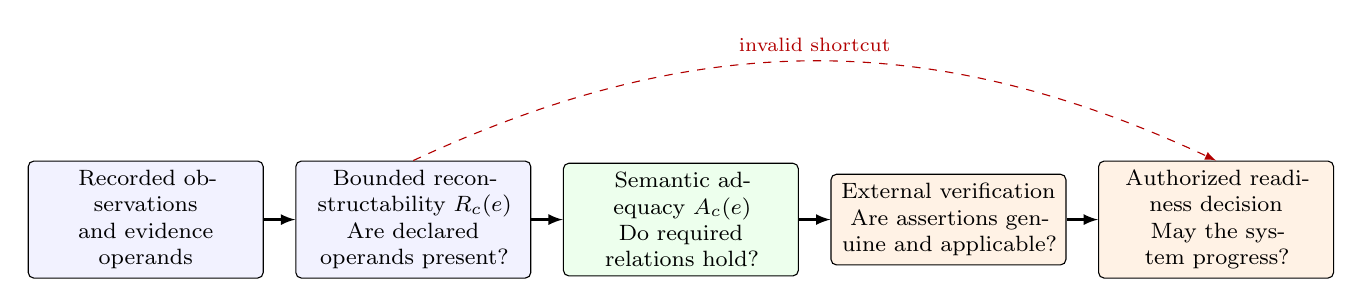
\begin{tikzpicture}[font=\footnotesize,>=latex,node distance=4mm]
  \tikzset{
    stage/.style={draw,rounded corners=2pt,align=center,text width=2.75cm,minimum height=11mm,fill=blue!5},
    gate/.style={draw,rounded corners=2pt,align=center,text width=2.75cm,minimum height=11mm,fill=green!7},
    authority/.style={draw,rounded corners=2pt,align=center,text width=2.75cm,minimum height=11mm,fill=orange!10}
  }
  \node[stage] (trace) {Recorded observations\\and evidence operands};
  \node[stage,right=of trace] (recon) {Bounded reconstructability $R_c(e)$\\Are declared operands present?};
  \node[gate,right=of recon] (adequacy) {Semantic adequacy $A_c(e)$\\Do required relations hold?};
  \node[authority,right=of adequacy] (truth) {External verification\\Are assertions genuine and applicable?};
  \node[authority,right=of truth] (decision) {Authorized readiness decision\\May the system progress?};
  \draw[->,thick] (trace) -- (recon);
  \draw[->,thick] (recon) -- (adequacy);
  \draw[->,thick] (adequacy) -- (truth);
  \draw[->,thick] (truth) -- (decision);
  \draw[red!70!black,dashed,->,bend left=25] (recon.north) to node[above,font=\scriptsize]{invalid shortcut} (decision.north);
\end{tikzpicture}
}
  \caption{A complete evidence representation remains upstream of semantic support, external verification, and an authorized readiness decision.}
  \label{fig:layers}
\end{figure}

\section{Related work}

\paragraph{Agent evidence and reconstructability.}
AgentTrace and OpenTelemetry define structured observations for agent and tool activity~\cite{alsayyad2026agenttrace,otel2026genai}; W3C PROV provides a general relational vocabulary for entities, activities, and agents~\cite{groth2013prov}. Work on agent execution provenance organizes sources, units, relations, representations, and trust functions~\cite{wang2026provenance}. Auditable-agent research similarly distinguishes action recovery, policy checkability, and evidence integrity~\cite{nian2026auditable}. Solozobov's Load-Bearing Evidence framework measures reconstructability across eight decision-property classes and explicitly notes that reconstructability is not correctness or safety~\cite{solozobov2026load}. We formalize one reason: an abstraction that retains availability but loses a claim relation is not label-separating.

\paragraph{Citation support and attribution faithfulness.}
Attributed-generation research evaluates whether cited passages support generated natural-language statements~\cite{gao2023alce}. Related RAG work distinguishes citation correctness from whether a generator actually relied on the cited document~\cite{wallat2024correctness}. The shared warning is that an attached reference is not sufficient by itself, but the tasks differ. Our label is a deterministic closed-profile predicate over structured evidence operands; it is not a judgment about text authorship, source relevance, or a model's causal reliance on a citation.

\paragraph{Behavioral and metamorphic evaluation.}
Metamorphic testing addresses cases where individual outputs are difficult to judge by specifying transformations and expected relations between executions~\cite{segura2016metamorphic}. CheckList applies capability- and behavior-oriented tests to expose failures hidden by aggregate accuracy~\cite{ribeiro2020checklist}. Mutation testing evaluates a test suite by deliberately changing program behavior~\cite{jia2011mutation}. Our matched pairs use the same experimental logic at the evidence layer: each mutation preserves structural availability while changing one claim-relevant relation. The goal is construct discrimination, not mutation-score comparison.

\paragraph{Reliability and decision authority.}
Agent reliability work argues that task success alone obscures consistency, robustness, predictability, and safety~\cite{rabanser2026reliability}. NIST's AI Risk Management Framework separates measurement from contextual risk treatment~\cite{nist2023airmf}. Runtime governance and verifier-determined sufficiency further distinguish transported assertions from relying-party decisions~\cite{kaul2026agentbound,macguire2026xchk}. Our authority boundary adopts this separation: local semantic support is evidence for a decision, not the decision itself.

\section{Matched-pair study}

\subsection{Research questions}

We ask: (RQ1) do practical agent-evidence profiles admit positive--negative pairs that are indistinguishable by required-field presence and JSON key/type shape? (RQ2) how many designed negatives remain false-supported as progressively richer value checks are added? (RQ3) are outputs reproducible and bounded against authority overclaiming?

\subsection{Profiles, provenance, and pair construction}

The system under study is the deterministic Python implementation of \code{saee.evaluate\_evidence}~\cite{saee2026artifact}. It loads one file-backed profile for each of four claims: resource authenticity, authorized agent action, human oversight, and execution boundary. The evaluator, profiles, and passing fixtures were committed at \code{be6ab57878dc7346da733e2f3b134aa3d3049af8} before construction of this study. The runner pins SHA-256 hashes for those components and stops on drift. This source-control separation reduces adaptive implementation risk, but does not remove white-box author bias.

The dataset contains 16 matched pairs, four per profile. Each starts from a canonical synthetic passing fixture. The negative replaces one existing scalar value, retaining every key, value type, and nominal descriptive outcome. Table~\ref{tab:pairs} summarizes the isolated conditions.

\begin{table}[t]
\centering
\caption{Relation-invalid member of each matched pair.}
\label{tab:pairs}
\small
\begin{tabularx}{\textwidth}{@{}llX@{}}
\toprule
Profile & Pair & Invalidated condition \\
\midrule
Resource & RA-01--04 & receipt digest; content digest; host binding; time order \\
Authorization & AA-01--04 & allow decision; authority window; scope; actor binding \\
Oversight & HO-01--04 & approval decision; time order; scope; action binding \\
Execution & EB-01--04 & receipt ref.; effect ref.; digest; resolved URI \\
\bottomrule
\end{tabularx}
\end{table}

The cases are intentionally easy to adjudicate and balanced by design. They are not sampled agent failures. Their purpose is to witness the equivalence classes in the corollaries while isolating relation families that occur in agent systems: equality bindings, temporal order, validity windows, scope coverage, digest consistency, and multi-object causal linkage.

\subsection{Baselines and evaluator}

We compare four deterministic rules:

\begin{description}
  \item[Field presence] supports iff every required field is non-empty.
  \item[Type and shape] additionally requires the complete JSON key/type signature to match the canonical positive fixture.
  \item[Decision-aware ablation] additionally requires \code{allow} for authorization and \code{approved} for oversight, but evaluates no cross-field relation.
  \item[Relation-aware profile] evaluates all declared profile relations and affirmative decision conditions.
\end{description}

The first two are provably unable to separate each pair. The third tests whether obvious decision semantics alone explain the negatives. The fourth is the existing system under study. Authored labels are positive for untouched fixtures and negative for mutations. We report confusion counts and, principally, false support among the 16 designed negatives. Classification rates describe only this constructed set.

The runner also checks pair count, claim balance, fixture allowlisting, path containment, replacement-only mutations, presence-vector equality, JSON-shape equality, expected reason codes, component hashes, and five-run determinism. A boundary violation is any output that asserts accountability, event occurrence, verified identity, verified authorization, a legal finding, or production readiness.

\subsection{Analysis status and statistical estimand}

This study is a retrospective frozen analysis, not a preregistered experiment. The 32 cases exhaust the authored dataset; they are not a random sample from an operational population. The primary quantities are exact finite-set counts: abstraction-equivalent pairs, false supports among the 16 designed negatives, agreement with authored labels and reason codes, and deterministic hash equality. All 16 pairs and all four rules are reported; no comparison was selected by a significance threshold.

Accordingly, we do not report $p$-values, confidence intervals, statistical power, or population accuracy. Those quantities would require a sampling frame or stochastic data-generating mechanism that this construct-validation design does not provide. Repetition checks computational determinism only; it does not create independent samples or sampling uncertainty.

\section{Results}

All 16 pairs have identical required-field presence vectors, identical JSON key/type signatures, and divergent semantic labels. Thus the 16 pairs instantiate the presence-equivalence corollary and require at least 16 errors from every presence-only classifier on this 32-case set.

Table~\ref{tab:results} shows the observed rules. Field presence and type/shape support all cases, causing 16 false supports. Checking affirmative decision values rejects AA-01 and HO-01, but still false-supports the remaining 14 relation-invalid cases. The relation-aware evaluator matches all 32 authored labels and expected reason-code lists. Its perfect result is construct validation on authored cases, not an estimate of unseen-case performance.

\begin{table}[t]
\centering
\caption{Confusion counts on 16 positive and 16 designed-negative cases.}
\label{tab:results}
\small
\begin{tabular}{@{}lrrrr@{}}
\toprule
Rule & TP & FP & TN & FN \\
\midrule
Field presence & 16 & 16 & 0 & 0 \\
Type and shape & 16 & 16 & 0 & 0 \\
Decision-aware ablation & 16 & 14 & 2 & 0 \\
Relation-aware profile & 16 & 0 & 16 & 0 \\
\bottomrule
\end{tabular}
\end{table}

\begin{figure}[t]
  \centering
  \resizebox{0.92\textwidth}{!}{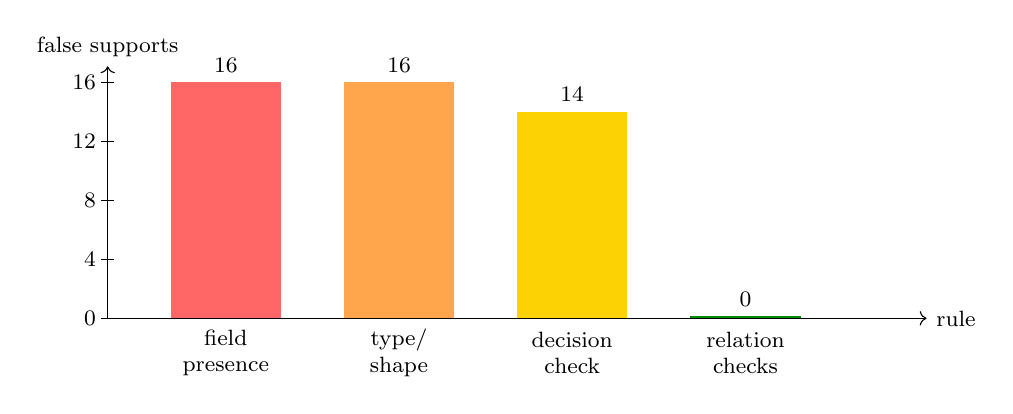
\begin{tikzpicture}[font=\footnotesize]
  \draw[->] (0,0) -- (10.4,0) node[right]{rule};
  \draw[->] (0,0) -- (0,3.2) node[above]{false supports};
  \foreach \y/\lab in {0/0,0.75/4,1.5/8,2.25/12,3/16} {
    \draw (-0.08,\y) -- (0.08,\y) node[left=3pt]{\lab};
  }
  \fill[red!60] (0.8,0) rectangle (2.2,3.0);
  \fill[orange!70] (3.0,0) rectangle (4.4,3.0);
  \fill[yellow!70!orange] (5.2,0) rectangle (6.6,2.625);
  \fill[green!55!black] (7.4,0) rectangle (8.8,0.03);
  \node[align=center] at (1.5,-0.44) {field\\presence};
  \node[align=center] at (3.7,-0.44) {type/\\shape};
  \node[align=center] at (5.9,-0.44) {decision\\check};
  \node[align=center] at (8.1,-0.44) {relation\\checks};
  \node[above] at (1.5,3.0) {16};
  \node[above] at (3.7,3.0) {16};
  \node[above] at (5.9,2.625) {14};
  \node[above] at (8.1,0.03) {0};
\end{tikzpicture}
}
  \caption{False supports among 16 designed relation-invalid cases.}
  \label{fig:false-support}
\end{figure}

Failure reasons localize the violated invariant: invalid receipt, non-allow decision, expired window, insufficient scope, actor mismatch, late approval, action mismatch, or invalid causal binding. This changes remediation. Missing evidence calls for collection; a relational failure calls for repair, renewed authority, or rejection.

Five repetitions produce the same result; the canonical SHA-256 begins \code{4d101bb8633e4acf}, with the full hash recorded in the result manifest. All 32 outputs retain the six protected authority fields as false. The runner makes no network request, reads no external resource, launches no subprocess, and executes no candidate code.

\section{Discussion}

\subsection{Implication for AI-agent evaluation}

The theorem turns a familiar warning---``complete does not mean correct''---into a design test. Before using an evidence abstraction for a claim, ask whether the claim label is constant inside every abstraction equivalence class. If not, either enrich the representation with the missing relation operands and checks or narrow the claim. Adding unrelated telemetry does not repair an expired delegation or mismatched digest.

The result also explains why aggregate evidence scores can be hazardous. A scalar may combine presence, integrity, provenance, and permission into one rank while discarding which invariant failed and who owns the next decision. An agent-readable evaluator should instead expose: the named profile, captured operands, evaluated relations, localized failures, unverified external assertions, and an explicit non-authorization statement. Those outputs allow a downstream agent to collect missing evidence, request applicable authority, repair provenance, or stop.

\subsection{What the study does and does not validate}

The matched pairs validate the existence and execution of a construct boundary across four profile families. Pre-existing evaluator code and pinned component hashes provide a stronger provenance story than building the classifier after seeing the cases. Nevertheless, the corresponding author knew the evaluator when designing mutations, reused one positive fixture per profile, and selected unambiguous failures. Zero errors therefore do not establish generalization, superiority, or deployment fitness.

A stronger follow-up should add independently authored cases, cross-harness traces, malformed-but-plausible packages, policy hierarchies, revoked credentials, and executed replay. It should pre-register relations and evaluate blinded holdout mutations. Population metrics become meaningful only when cases are sampled from a defined operational distribution.

\subsection{Threats to validity}

\paragraph{Construct validity.}
Bounded reconstructability covers field presence under four local profiles; it does not implement the eight-property Load-Bearing Evidence metric, trace fidelity, causal identification, or replay. Exact equality is used for scope coverage, so richer policy lattices remain untested.

\paragraph{Internal validity.}
The experiment is white-box and synthetic. It performs no model fitting, hyperparameter search, train/test split, or test-set selection, so conventional predictive-model leakage is not the relevant threat. The relevant threat is target-aware case selection: the corresponding author knew the evaluator, profiles, and fixtures while designing mutations. Committed evaluator provenance prevents post-hoc code adaptation in this artifact, but it does not remove case-selection bias. The relation-aware result is therefore a regression result, not a blinded holdout or unbiased benchmark.

\paragraph{External validity.}
No live agent run, human participant, customer record, or external identity system is involved. The balanced class ratio is artificial. Deterministic hashes in one environment do not prove portability across all platforms.

\paragraph{Authority validity.}
Profile support is not external verification or permission. A complete and semantically consistent package may still cite a fabricated identity, revoked delegation, inapplicable policy, or false event. The evaluator also cannot determine whether text was written by a human or AI, legal authorship or copyright ownership, academic misconduct, or editorial sanctions. The actual relying party must retain the readiness decision.

\paragraph{Ethics and privacy.}
The study uses synthetic JSON packages only. It includes no human participants, interventions, personal or health records, customer data, live agent interactions, or external identity lookups. Ethics approval and informed consent are therefore not applicable to this study design. Author contact metadata used for publication administration is separate from the experimental dataset and is not included in the reproducibility artifact.

\section{Conclusion}

Evidence availability is indispensable for evaluating consequential AI-agent behavior, but it is a representation, not a verdict. Theorem~1 establishes that a classifier can perfectly recover a semantic claim from an evidence abstraction exactly when the abstraction separates differently labelled packages. When field presence or JSON shape collapses a valid and relation-invalid package into the same value, no classifier over that abstraction can classify both correctly.

Sixteen matched pairs make this boundary executable. Structural completeness false-supports every designed negative; affirmative decision checks remove only two; relation-aware predicates separate the authored cases and explain each rejection. The practical stop rule is concise: a readiness classifier must consume a representation that preserves every relation on which its claim depends, and its output must not usurp external verification or decision authority.

\section*{Data and code availability}
The dataset, data dictionary, retrospective analysis plan, pinned environment, runner, expected results, full result manifest, and verification instructions are supplied as supplementary material with this manuscript. The referenced evaluator snapshot is available at commit \code{f6ac41f4b068377e7778e8c3d83b99bd8382debc}~\cite{saee2026artifact}. The supplementary artifact remains a controlled synthetic study and contains no personal or production data.

\section*{CRediT authorship contribution statement}
Bin Zhang: Conceptualization, Methodology, Software, Validation, Formal analysis, Investigation, Data curation, Visualization, Writing -- original draft, Writing -- review and editing.

Xiaojuan Sun: Conceptualization, Investigation, Data curation, Resources.

\section*{Funding}
This research received no specific grant from any funding agency in the public, commercial, or not-for-profit sectors.

\section*{Declaration of competing interest}
The authors declare that they have no known competing financial interests or personal relationships that could have appeared to influence the work reported in this paper.

\section*{Declaration of generative AI and AI-assisted technologies in the manuscript preparation process}
During preparation of this work, the corresponding author used OpenAI Codex for literature-search assistance, experiment implementation, manuscript drafting and editing, and verification. The corresponding author reviewed and verified the resulting code, references, analysis, and text. All authors reviewed and approved the final disclosure and manuscript.

\small
\setlength{\bibsep}{1pt}
\bibliographystyle{elsarticle-num-names}
\bibliography{references}

\end{document}
